\documentclass{beamer}
\usetheme{Warsaw}
\usepackage{lmodern}
\usepackage[french]{babel}
\usepackage[T1]{fontenc}
\usepackage[utf8]{inputenc}
\usepackage{graphicx}

\begin{document}
\title{}
\title{\textbf{Soutenance SIG}}
\author[FONTORBE, FRANÇOIS, MOROSI, PERRIN]{
	\textit{Jordan FONTORBE}\\
	\textit{Willy FRANÇOIS}\\
	\textit{Jérémy MOROSI}\\
	\textit{Jean-Baptiste PERRIN}
}
\maketitle

\tableofcontents

\section{Réalisation}

\subsection{Commun}
\subsubsection{Package data}
\begin{frame}
\frametitle{Package data}

Le modèle :\\
\begin{columns}
\begin{column}{.49\textwidth}
\begin{block}{Bases}
\begin{itemize}
\visible<1->{
\item Node : une latitude et longitude
}
\visible<2->{
\item Road : une liste de noeud, un type (route, chemin, etc.)
}
\end{itemize}
\end{block}
\end{column}
\begin{column}{.49\textwidth}
\visible<3->{
\begin{block}{Structure: nom, liste de noeuds}
\begin{itemize}
\item Building : liste de trous
\item Basin
\item Forest
\item Hole : la structure auquel il appartient
\end{itemize}
\end{block}
}
\end{column}
\end{columns}
\end{frame}

\subsection{Arbre de décision}

\begin{frame}
\frametitle{Arbre de décision}
\begin{block}{Arbre de décision}
\begin{itemize}
\item Un noeud racine
\item Noeuds décomposés en quatre noeuds
\item Terminé par des feuilles
\end{itemize}
\end{block}
\end{frame}

\begin{frame}
\frametitle{Arbre de décision}
\begin{block}{Noeud}
\begin{itemize}
\item Des coordonnées $(x, y)$
\item Quatre sous-noeuds:\begin{itemize}
\item En haut à gauche
\item En haut à droite
\item En bas à gauche
\item En bas à droite
\end{itemize}
\end{itemize}
\end{block}
\end{frame}

\begin{frame}
\frametitle{Arbre de décision}
\begin{block}{Noeud}
\begin{itemize}
\item Liste de bâtiments:\begin{itemize}
\item Rectangle englobant du bâtiment
\item Identifiant du bâtiment
\end{itemize}
\end{itemize}
\end{block}
\end{frame}

\begin{frame}
\frametitle{Arbre de décision}
\begin{block}{Complexité}
\begin{itemize}
\item Un noeud n'existe que si il possède une feuille
\item Une feuille n'existe que si elle possède un bâtiment
\item Découpage en grille de la carte
\item Rectangle englobant
\end{itemize}
\end{block}
\end{frame}

\begin{frame}
\begin{figure}
\centering
\resizebox{0.75\linewidth}{!}{
\includegraphics{../images/modeleArbreDecision.pdf}
}
\caption{Arbre de décision}
\end{figure}
\end{frame}

\subsection{WebService}
\begin{frame}
\frametitle{WebService}
\begin{block}{Méthodes nécessaires pour le mode `remote'}
\begin{itemize}
\item Récupération de la map (format XML)
\item Récupération d'un bâtiment à partir de coordonnées (format JSON)
\item Récupération d'un itinéraire à partir d'un bâtiment de départ et d'arrivée (format JSON)
\end{itemize}
\end{block}
\end{frame}

\begin{frame}
\begin{figure}
\centering
\resizebox{\linewidth}{!}{
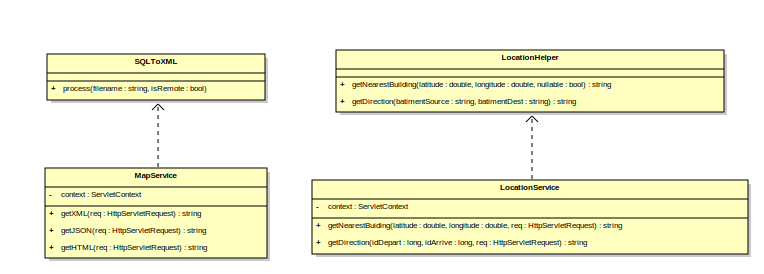
\includegraphics{../images/webService.pdf}
}
\caption{Web Service}
\end{figure}
\end{frame}

\subsection{Android}
\begin{frame}
\frametitle{Android}
\begin{block}{ActivityBase}
\begin{itemize}
\item Affichage de la carte
\item Réception des données du GPS
\item Lien entre l'utilisateur et l'affichage
\end{itemize}
\end{block}
\begin{block}{ISig1337}
\begin{itemize}
\item Méthodes communes pour récupérer:\begin{itemize}
\item Les éléments (bâtiments, routes...)
\item Le bâtiment à partir de coordonnées
\item L'itinéraire entre deux bâtiments
\end{itemize}
\end{itemize}
\end{block}
\end{frame}

\begin{frame}
\frametitle{Android}
\begin{block}{LocalActivity}
\begin{itemize}
\item Utilise LocalSig1337
\end{itemize}
\end{block}
\begin{block}{LocalSig1337}
\begin{itemize}
\item Implémente les méthodes de l'interface en:\begin{itemize}
\item Utilisant l'arbre de décision
\item Utilisant le graphe
\end{itemize}
\end{itemize}
\end{block}
\end{frame}

\begin{frame}
\frametitle{Android}
\begin{block}{RemoteActivity}
\begin{itemize}
\item Utilise RemoteSig1337
\end{itemize}
\end{block}
\begin{block}{RemoteSig1337}
\begin{itemize}
\item Implémente les méthodes de l'interface en:\begin{itemize}
\item Appelant le WebService
\end{itemize}
\end{itemize}
\end{block}
\end{frame}

\begin{frame}
\begin{figure}
\centering
\resizebox{\linewidth}{!}{
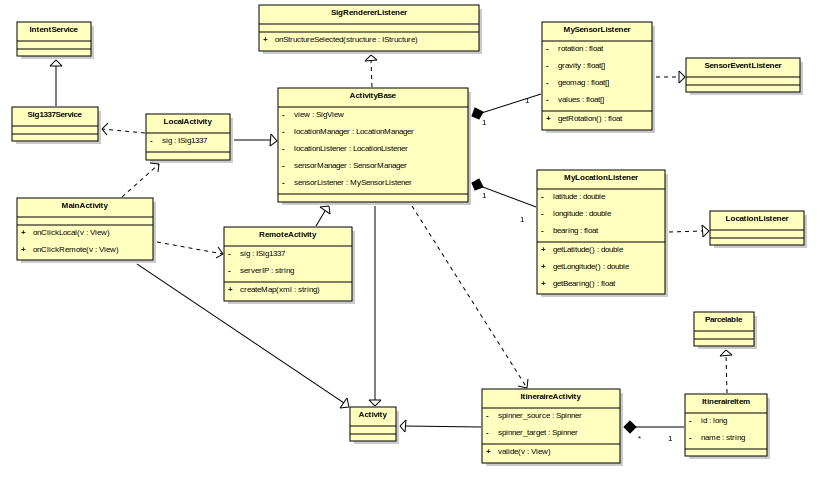
\includegraphics{../images/androidActivity.pdf}
}
\caption{Architecture android}
\end{figure}
\end{frame}


\section{Difficultés rencontrées}
\begin{frame}
\frametitle{Difficultés rencontrées}
\begin{alertblock}{$\underline{/\hat{!}\backslash}$}
\begin{itemize}
\item Import des données OpenStreetMap
\item Arbre de décision
\item Itinéraire en local
\end{itemize}
\end{alertblock}
\end{frame}


\section{Conclusion}
\begin{frame}
\end{frame}


\end{document}
